% #############################################################################
% This is Chapter 3
% !TEX root = ../main.tex
% #############################################################################
% Change the Name of the Chapter i the following line
\fancychapter{Related Work}
\cleardoublepage
% The following line allows to ref this chapter
\label{chap:architecture}

This chapter reviews existing work in aerial image segmentation datasets, ranging from traditional semantic and instance segmentation datasets to specialized referring segmentation datasets and historical imagery applications. It then surveys architectures for Referring Remote Sensing Instance Segmentation (RRSIS), including approaches built on vision-language encoders (e.g., CLIP, SigLIP) and promptable segmentation decoders (e.g., SAM), as well as RSRefSeg-style bridging designs (Section~3.2).

% #############################################################################
\section{Aerial Image Segmentation Datasets}

The foundation for effective aerial image understanding lies in comprehensive datasets that capture the diversity and complexity of remote sensing imagery. This section examines the evolution from traditional segmentation datasets to specialized referring segmentation datasets and historical imagery applications.

\subsection{Traditional Aerial Segmentation Datasets}

Early efforts in aerial image segmentation focused on providing basic semantic and instance annotations for common remote sensing tasks. These foundational datasets established important benchmarks and annotation standards that continue to influence modern dataset construction.

The iSAID dataset~\cite{zamir2019isaid} represents a significant advancement in instance segmentation for aerial imagery, providing detailed object-level annotations across diverse geographical regions. Building upon the DOTA dataset foundation~\cite{xia2018dota}, iSAID offers precise instance boundaries for 15 different categories commonly found in aerial imagery, including vehicles, buildings, and infrastructure elements. The dataset contains over 655,000 annotated instances across high-resolution imagery, establishing a comprehensive benchmark for instance-level understanding in remote sensing applications. Example annotations are shown in Figure~\ref{fig:isaid_examples}. Key characteristics are summarized in Table~\ref{tab:source_comparison}.

\begin{figure}[htbp]
\centering
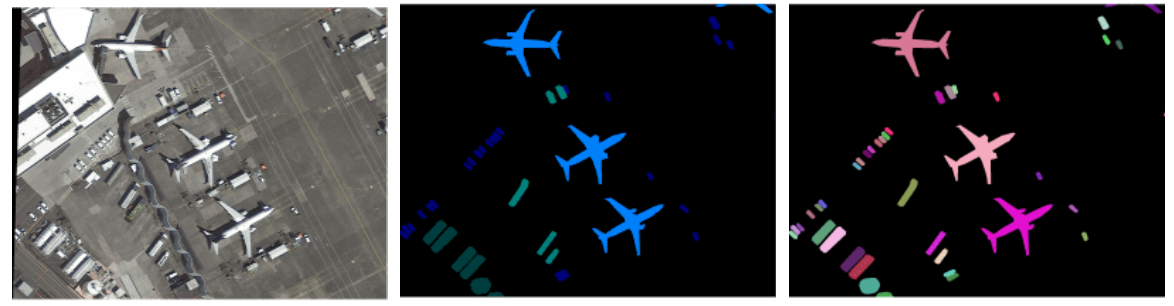
\includegraphics[width=0.8\textwidth]{Images/isaid_examples.png}
\caption{iSAID dataset examples showing instance segmentation annotations for aerial imagery, demonstrating the detailed object-level boundaries across diverse geographical contexts.}
\label{fig:isaid_examples}
\end{figure}

The LoveDA dataset~\cite{wang2021loveda} takes a complementary approach, focusing on semantic segmentation for land cover and infrastructure analysis. Unlike instance-based approaches, LoveDA provides dense pixel-level annotations for seven primary land cover categories including buildings, roads, water, barren land, forest, agriculture, and background. The dataset emphasizes multi-domain applicability by incorporating both urban and rural imagery collected from different geographical regions, enabling research into domain adaptation techniques for aerial image analysis. Representative samples appear in Figure~\ref{fig:loveda_examples}. Key characteristics are summarized in Table~\ref{tab:source_comparison}.

\begin{figure}[htbp]
\centering
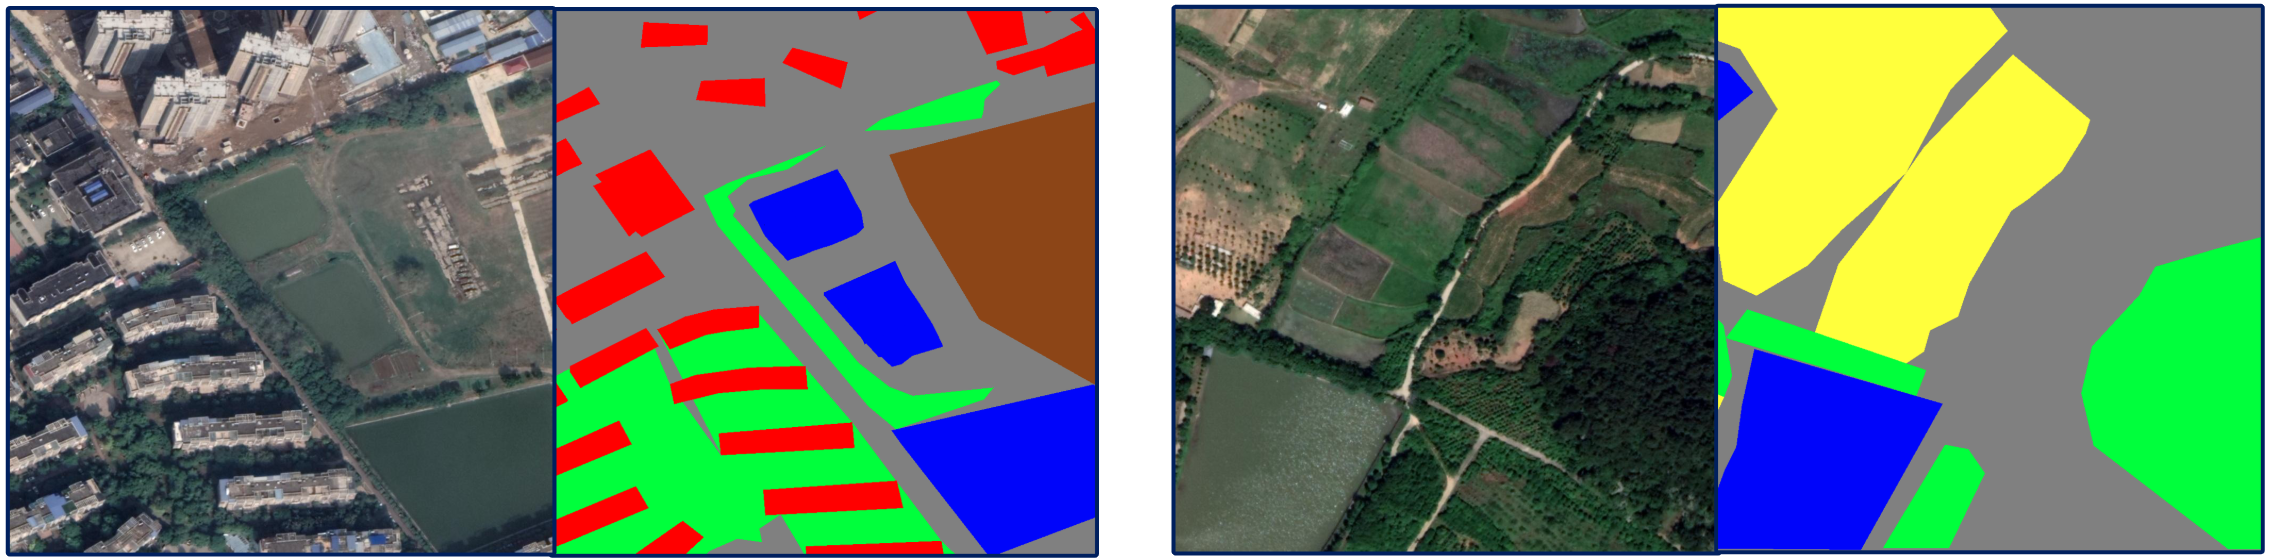
\includegraphics[width=0.8\textwidth]{Images/loveda.png}
\caption{LoveDA dataset examples showing semantic segmentation annotations for land use and land cover classification, highlighting the dense pixel-level labeling approach across urban and rural contexts.}
\label{fig:loveda_examples}
\end{figure}

\subsection{Referring Segmentation Datasets}

Traditional segmentation datasets provide important foundations, but they lack the natural language interface necessary for interactive aerial image analysis. Referring segmentation datasets address this limitation by combining visual annotations with natural language descriptions, enabling text-guided segmentation capabilities.

RefSegRS~\cite{chen2025rsrefseg} pioneered the field of referring segmentation for remote sensing imagery, introducing the first dataset to combine aerial imagery with natural language referring expressions. Built upon the SkyScapes dataset foundation, RefSegRS contains 4,420 triplets of images, referring expressions, and corresponding segmentation masks. The dataset focuses on establishing basic referring segmentation capabilities for aerial imagery, with expressions emphasizing spatial relationships, object attributes, and contextual descriptions that are characteristic of remote sensing analysis workflows. Example samples are illustrated in Figure~\ref{fig:aerial_datasets}.

RRSIS-D~\cite{yuan2023rrsis} expanded upon the RefSegRS foundation by introducing larger scale and semi-automated annotation approaches. The dataset contains 17,402 triplets derived from the RSVGD dataset, incorporating Segment Anything Model (SAM) assistance to accelerate annotation generation while maintaining quality standards. RRSIS-D addresses scale limitations of earlier datasets while introducing more diverse expression types across 20 different object categories and seven attribute dimensions, enabling more comprehensive evaluation of referring segmentation approaches. Visual examples appear in Figure~\ref{fig:aerial_datasets}. Comparative statistics across referring datasets are provided in Table~\ref{tab:rrsis_comparison}.

\begin{figure}[htbp]
\centering
\subfigure[RefSegRS dataset example samples.]{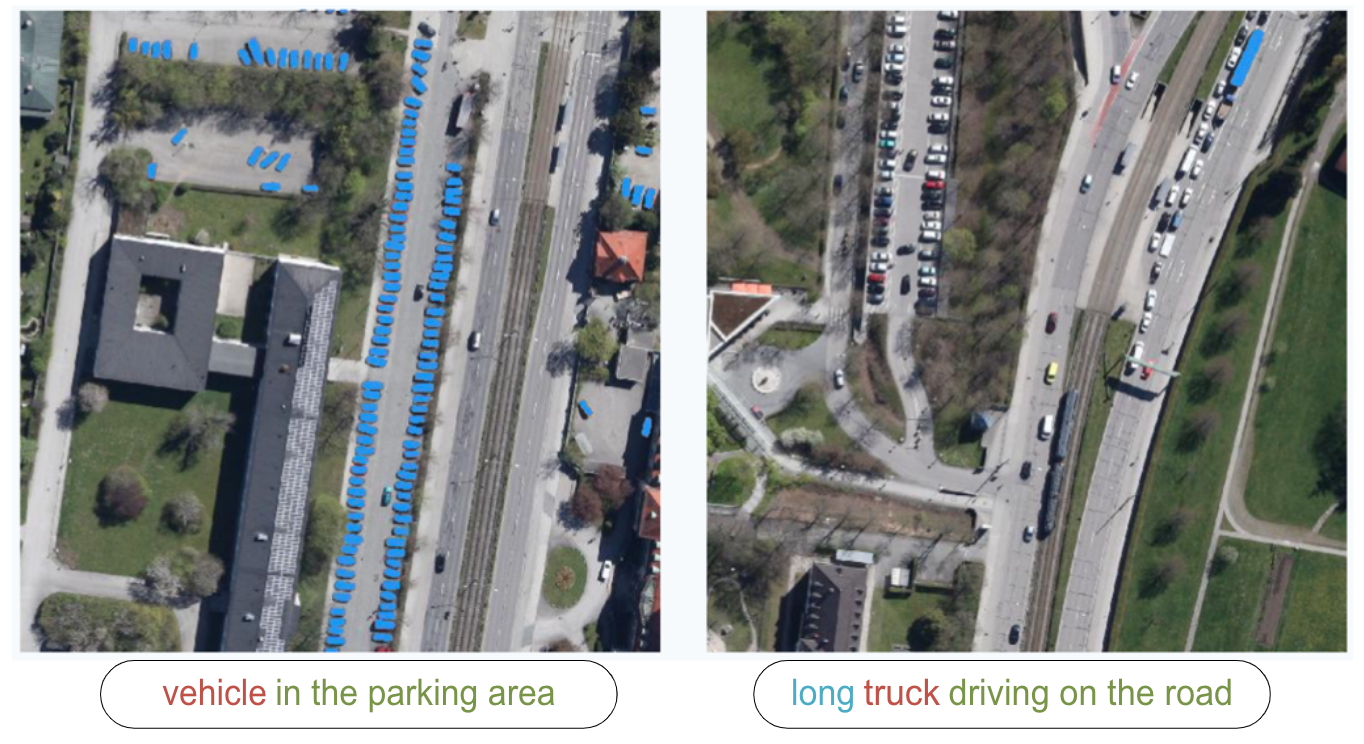
\includegraphics[width=0.45\textwidth]{Images/refsegrs.png}\label{fig:refsegrs}}
\hfill
\subfigure[RRSIS-D dataset example samples.]{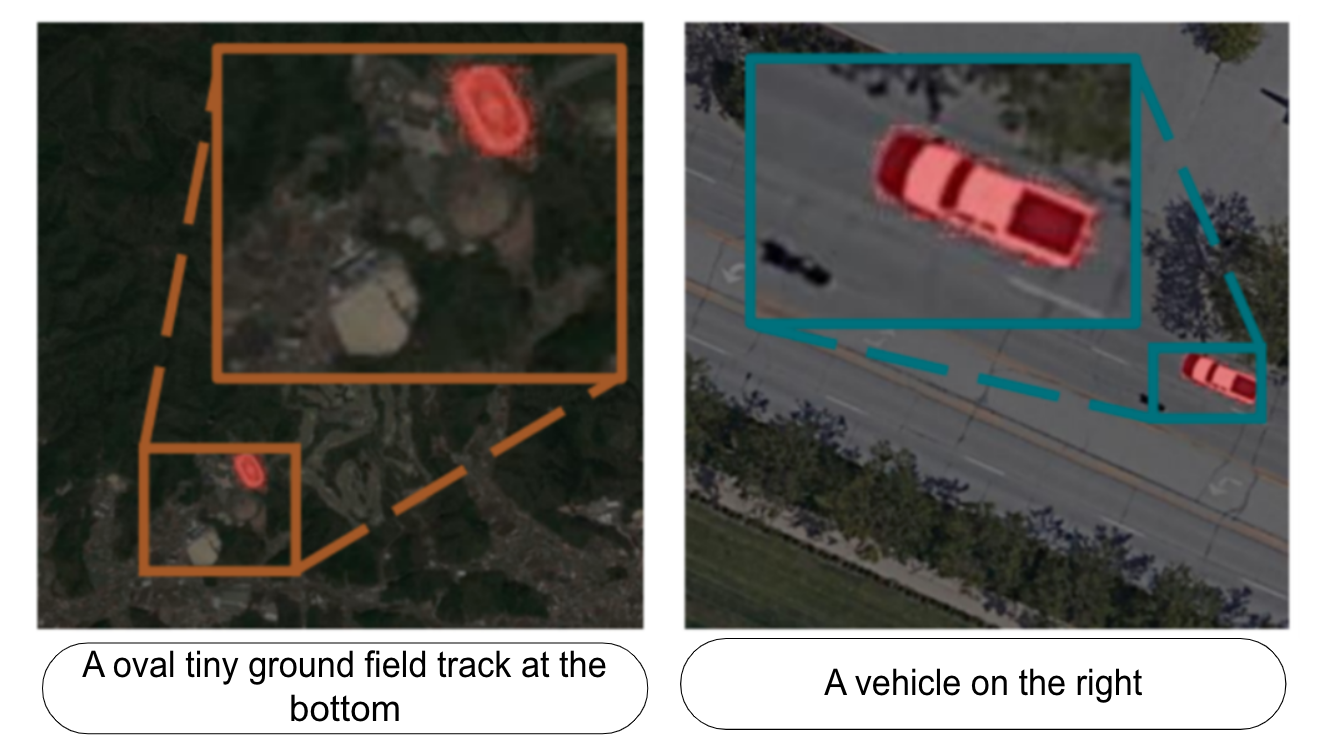
\includegraphics[width=0.45\textwidth]{Images/rrsisd.png}\label{fig:rrsisd}}
\caption{Examples from early aerial referring segmentation datasets showing the evolution from basic referring expressions to more diverse and comprehensive annotation approaches.}
\label{fig:aerial_datasets}
\end{figure}

NWPU-Refer~\cite{yang2024large} represents the current state-of-the-art in aerial referring segmentation datasets, significantly expanding both scale and annotation sophistication. The dataset contains 49,745 triplets sourced from multiple global aerial imagery collections, providing comprehensive coverage across different geographical regions and imaging conditions. NWPU-Refer introduces enhanced annotation quality through purely manual annotation processes, resulting in more natural and diverse referring expressions. The dataset incorporates 32 object categories with six attribute dimensions, enabling evaluation of fine-grained referring segmentation capabilities that closely match real-world aerial image analysis requirements. Comparative statistics are shown in Table~\ref{tab:rrsis_comparison}.

\subsection{Historical Imagery Segmentation}

While contemporary aerial datasets provide important foundations for modern remote sensing analysis, historical imagery represents a largely unexplored domain with significant research and practical value. Historical aerial imagery offers unique insights into temporal changes in land use, urban development patterns, and environmental evolution that cannot be captured through contemporary imagery alone. However, the scarcity of annotated historical datasets has limited progress in this important application area.

The UrbanSatSeg1960 dataset~\cite{hao2025urban1960satseg} addresses this gap by providing semantic segmentation annotations for historical urban aerial imagery from the 1960s era. This specialized dataset focuses on urban environments captured during a pivotal period of global urbanization, offering ground truth annotations for land cover categories relevant to historical analysis including buildings, roads, vegetation, and open spaces. UrbanSatSeg1960 enables research into historical imagery understanding while providing essential training data for temporal analysis applications that require consistent segmentation capabilities across different imaging eras. Representative imagery appears in Figure~\ref{fig:historical_examples}.

\begin{table}[htbp]
\centering
\caption{Historical Imagery Dataset Summary}
\label{tab:historic_comparison}
\begin{tabular}{@{}ll@{}}
\toprule
\textbf{Feature} & \textbf{Urban1960SatSeg} \\
\midrule
Size & N/A \\
Source & 1960s urban aerial imagery \\
Annotation & Semantic segmentation (historical scenes) \\
Resolution & Variable \\
Focus & Historic urban land-cover segmentation \\
Categories & Buildings, roads, vegetation, open spaces \\
\bottomrule
\end{tabular}
\end{table}

\begin{figure}[htbp]
\centering
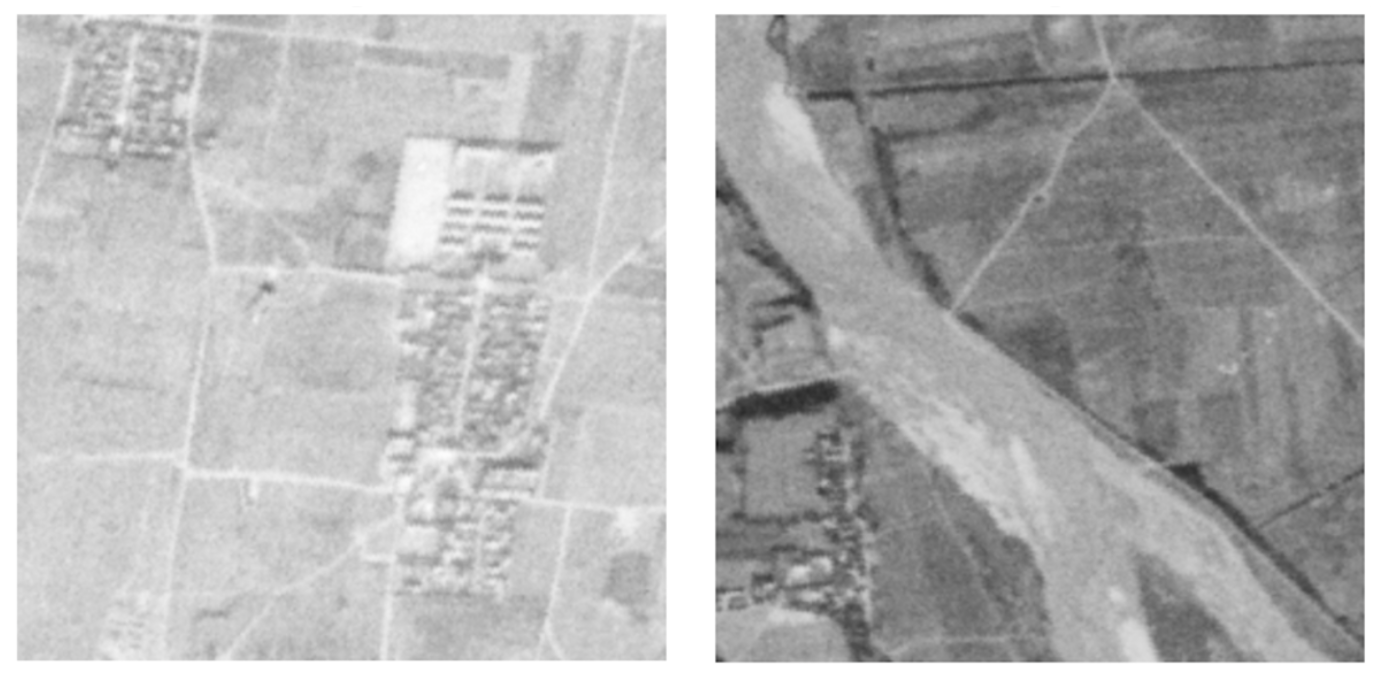
\includegraphics[width=0.6\textwidth]{Images/1960.png}
\caption{Historical aerial imagery examples from the UrbanSatSeg1960 dataset showing the characteristic visual properties of 1960s aerial photography, including reduced contrast, grayscale capture, and period-specific urban development patterns.}
\label{fig:historical_examples}
\end{figure}

\begin{table}[htbp]
\centering
\caption{Source Aerial Dataset Comparison}
\label{tab:source_comparison}
\begin{tabular}{@{}lll@{}}
\toprule
\textbf{Feature} & \textbf{iSAID} & \textbf{LoveDA} \\
\midrule
Size & 655,451 instances & 5,987 images \\
Source & DOTA (re-ann.) & Spaceborne (0.3m) \\
Annotation & Professional & Manual \\
Resolution & High res. & 1024×1024px \\
Focus & Instance Seg. & Land-cover Seg. + UDA \\
Categories & 15 & 7 \\
Attributes & - & Domain labels \\
\bottomrule
\end{tabular}
\end{table}

\begin{table}[htbp]
\centering
\caption{Aerial Referring Segmentation (RRSIS) Dataset Comparison}
\label{tab:rrsis_comparison}
\begin{tabular}{@{}llll@{}}
\toprule
\textbf{Feature} & \textbf{RefSegRS} & \textbf{RRSIS-D} & \textbf{NWPU-Refer} \\
\midrule
Size & 4,420 triplets & 17,402 triplets & 49,745 triplets \\
Source & SkyScapes & RSVGD & Multi-source global \\
Annotation & Manual & Semi-auto (SAM) & Manual \\
Resolution & Limited & 800×800 fixed & 1024-2048px \\
Focus & RRSIS & RRSIS & RRSIS \\
Categories & - & 20 & 32 \\
Attributes & 3 & 7 & 6 dimensions \\
\bottomrule
\end{tabular}
\end{table}


% #############################################################################
\section{Architectures for RRSIS}

Architectures for referring segmentation in aerial imagery follow two broad paths. One family builds specialized networks tailored to overhead scenes, emphasizing multi-scale fusion and rotation handling without relying on large vision-language backbones. A second family leverages foundation models—vision encoders (e.g., CLIP~\cite{clip} or SigLIP~\cite{siglip,siglip2}) and segmentation decoders (e.g., SAM~\cite{sam})—and focuses on bridging text-vision semantics for mask prediction. This section outlines representative approaches from both lines of work.

By the same authors who introduced the RRSIS-D dataset, the Rotated Multi-Scale Interaction Network (RMSIN) exemplifies the specialized-network path~\cite{liu2024rotated}. It introduces three modules—Intra-scale Interaction (IIM) for fine-grained detail, Cross-scale Interaction (CIM) for multi-resolution fusion, and Adaptive Rotated Convolution (ARC) for orientation variation—achieving improvements over strong baselines and showing the value of remote-sensing-specific inductive biases. This reflects a cohesive benchmark-method pairing within that line of work.

From the same authors who released the NWPU-Refer dataset, MRSNet advances the specialized-network line with intra-scale and hierarchical feature interaction modules designed to better capture multi-scale context in overhead scenes, mirroring the benchmark-method linkage seen with RMSIN and RRSIS-D. These specialized approaches emphasize bespoke inductive biases tailored specifically for the unique challenges of aerial imagery analysis.

In contrast, foundation-model approaches emphasize powerful pretrained backbones and light semantic bridging, trading bespoke inductive biases for transfer from large-scale pretraining. These approaches leverage the substantial progress in vision-language models and segmentation foundations to achieve strong performance through parameter-efficient adaptation.

Vision-language models such as CLIP~\cite{clip} establish crucial connections between visual and textual modalities through contrastive learning, enabling zero-shot classification capabilities that transfer effectively to aerial imagery domains. The learned joint embedding spaces capture semantic relationships that prove valuable for understanding aerial scene content and object categories. SigLIP~\cite{siglip,siglip2} represents an advancement in vision-language training methodologies, improving upon CLIP's contrastive approach through more efficient training objectives and enhanced representation learning. These improvements translate to better performance on downstream aerial image understanding tasks where precise visual-textual alignment is critical.

The Segment Anything Model (SAM) provides a foundational approach to semantic segmentation through its prompt-based architecture, as illustrated in Figure~\ref{fig:sam_architecture}~\cite{sam}. SAM's design incorporates three key components that work in concert to achieve exceptional segmentation performance across diverse domains. The image encoder processes input imagery into rich hierarchical feature representations using a Vision Transformer (ViT) backbone, capturing both fine-grained details and global context essential for understanding complex aerial scenes. The prompt encoder handles various input modalities including points, boxes, and masks, transforming these diverse prompt types into unified embedding representations that guide the segmentation process. The mask decoder utilizes these image and prompt embeddings through a sophisticated attention mechanism to generate precise segmentation boundaries, producing multiple candidate masks with confidence scores that enable robust target selection.

This architecture demonstrates remarkable generalization capabilities across diverse image domains, including aerial imagery, where its ability to process multiple prompt types enables flexible segmentation workflows that can adapt to different user requirements and annotation strategies. The model's foundation training on massive datasets provides strong zero-shot capabilities for aerial imagery, while its prompt-based design allows for interactive refinement of segmentation results through iterative point or box inputs.

\begin{figure}[htbp]
\centering
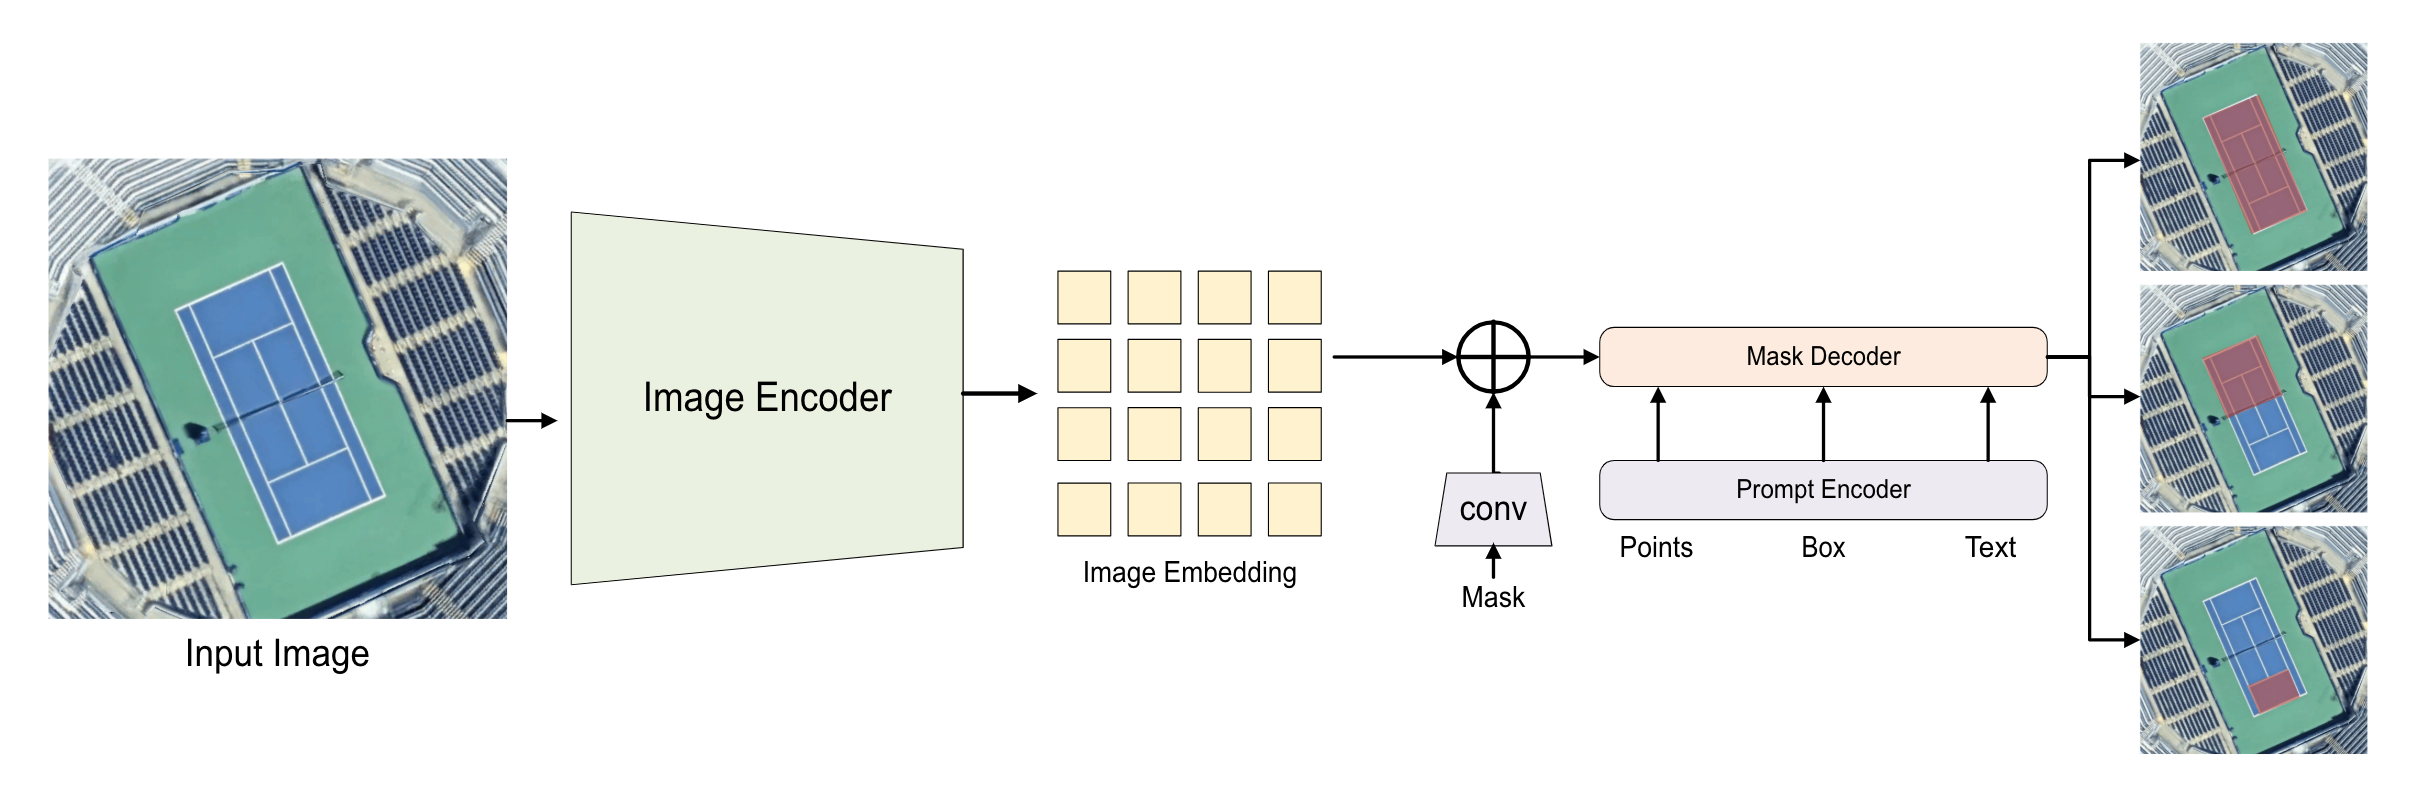
\includegraphics[width=1.0\textwidth]{Images/sam.png}
\caption{Segment Anything Model (SAM) architecture showing the image encoder, prompt encoder, and mask decoder components. The model processes various prompt types including points, boxes, and text to generate precise segmentation masks with hierarchical feature processing and attention-based mask generation.}
\label{fig:sam_architecture}
\end{figure}

RSRefSeg~\cite{chen2025rsrefseg} represents the foundation-model path by coupling a vision-language encoder with a segmentation decoder via a learned prompting bridge mechanism. As shown in Figure~\ref{fig:rsrefseg_architecture}, the architecture integrates SigLIP vision-language encoders with SAM mask decoders through custom prompter networks that convert text semantics into decoder-friendly prompts.

The architecture addresses the fundamental challenge of bridging text-vision semantics for precise mask prediction in aerial imagery. The SigLIP encoder processes both the input aerial image and the referring expression, creating aligned representations in a joint embedding space. This vision-language understanding provides the semantic foundation necessary for distinguishing between visually similar objects based on their textual descriptions.

The critical innovation lies in the AttnPrompter mechanism, which serves as the bridge between the vision-language understanding and the segmentation generation. This component transforms the text-aligned visual features into the specific prompt formats required by SAM's architecture. The dual-pathway design processes both local token-level and global sentence-level text-visual interactions, generating both sparse prompts (such as point and box coordinates) and dense prompts (such as mask embeddings) that guide SAM's mask decoder toward the target object described in the referring expression.

SAM's mask decoder receives these carefully constructed prompts and leverages its pretrained segmentation capabilities to generate precise object boundaries. The decoder's attention mechanisms utilize the semantic guidance provided by the prompter to focus on the relevant regions within the aerial image, producing high-quality segmentation masks that accurately capture the boundaries of the referred object even in complex aerial scenes with high object density and varying scales.

This foundation-model approach achieves strong performance through parameter-efficient fine-tuning strategies such as LoRA (Low-Rank Adaptation)~\cite{lora}, which enables effective task-specific adaptation while preserving the powerful pretrained representations learned during foundation model training. The architecture addresses the unique challenges of aerial imagery analysis, including varied object scales, complex spatial relationships, and domain-specific terminology requirements, while benefiting from the robust generalization capabilities inherited from its foundation model components.

\begin{figure}[H]
\centering
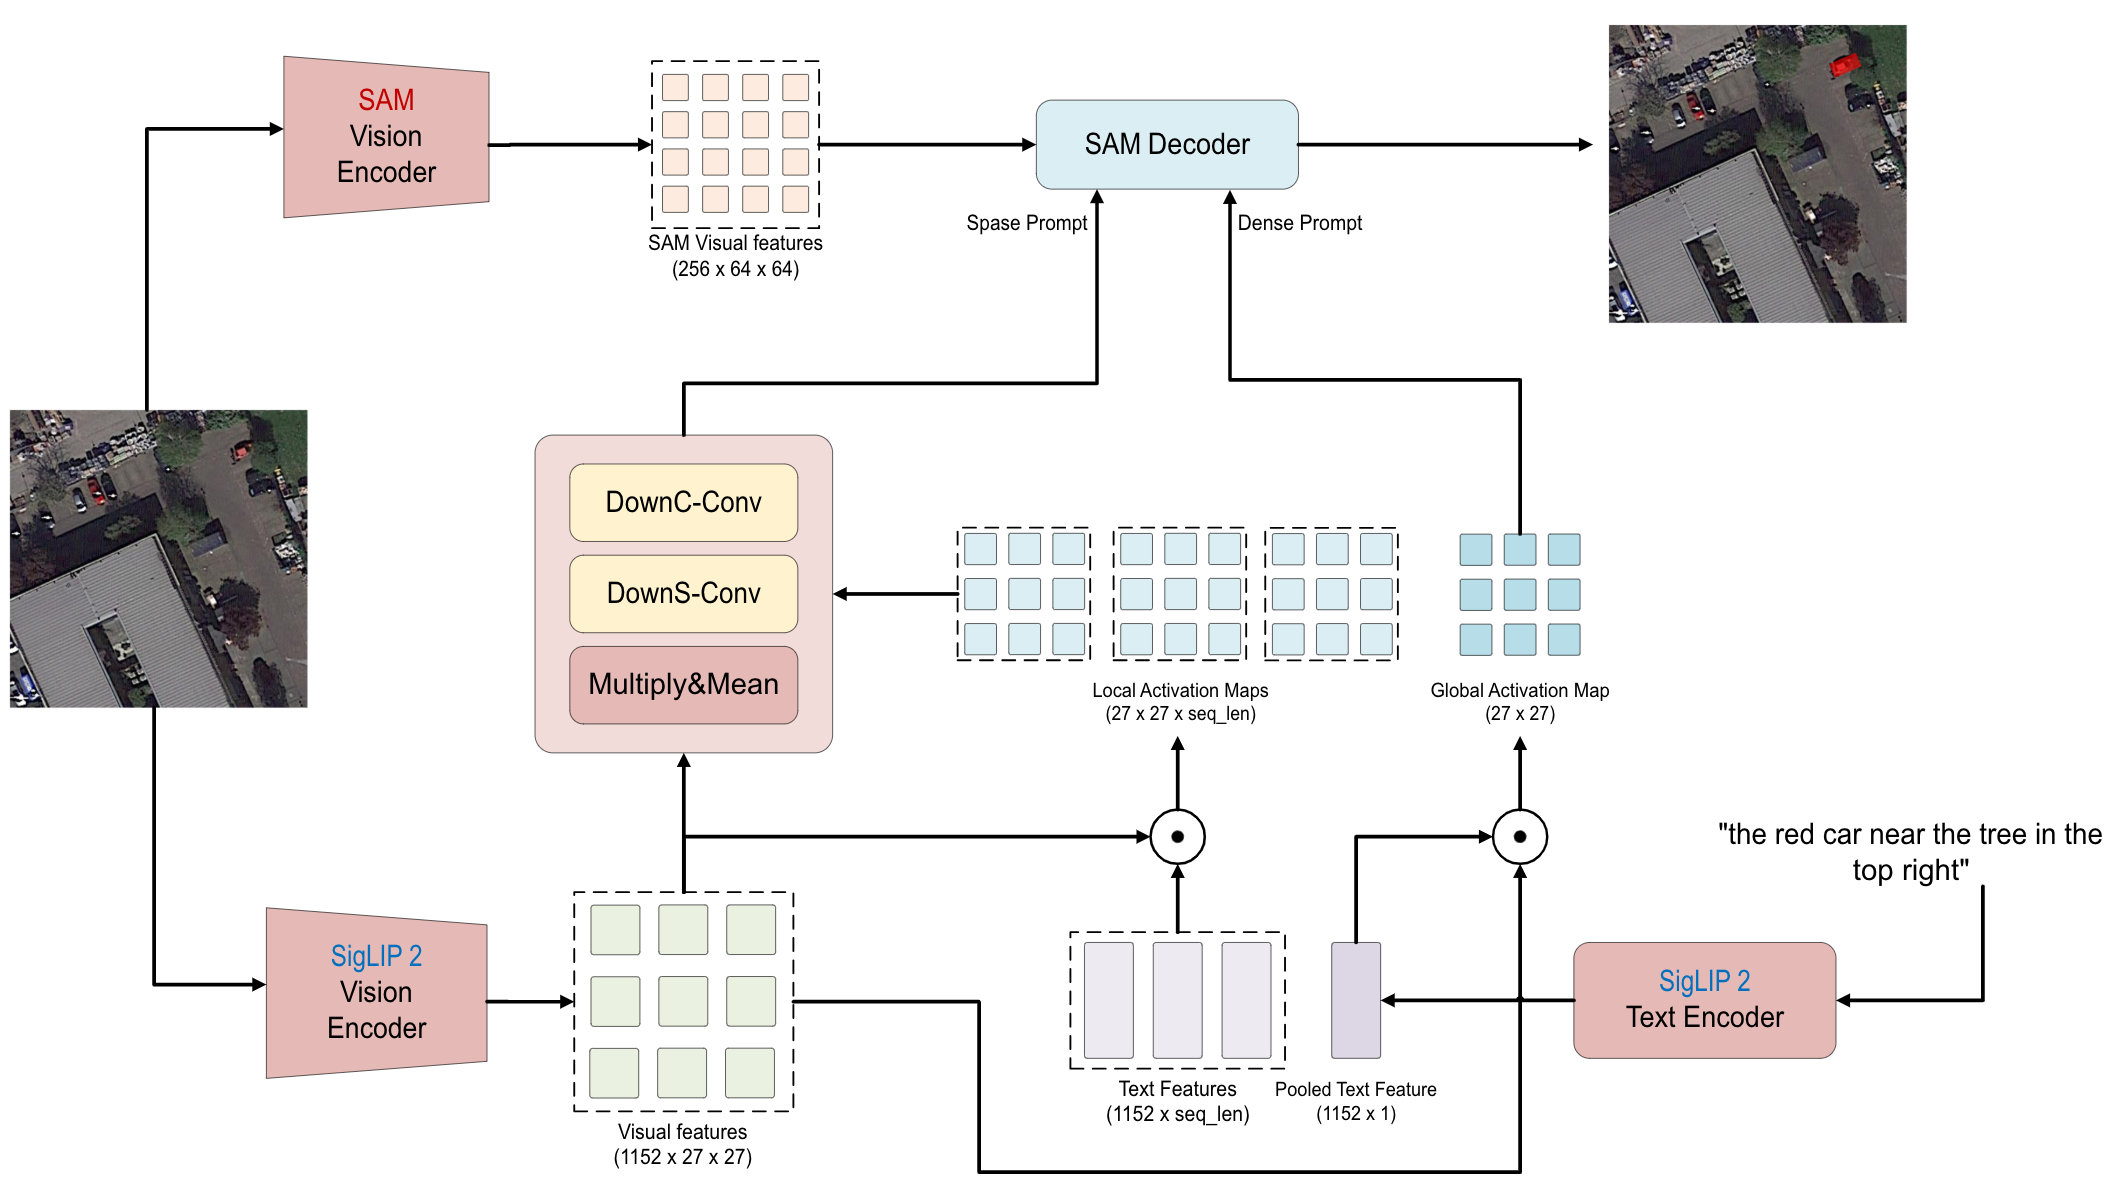
\includegraphics[width=\textwidth]{Images/clipsam.png}
\caption{RSRefSeg architecture overview showing the integration of SigLIP vision-language encoder with SAM mask decoder through the AttnPrompter bridging mechanism. The dual-pathway design processes both local (token-level) and global (sentence-level) text-visual interactions to generate sparse and dense prompts for precise aerial image segmentation guided by natural language descriptions.}
\label{fig:rsrefseg_architecture}
\end{figure}

% #############################################################################
\section{Overview}

The current landscape of aerial image segmentation is shaped by three pillars that enable language-guided segmentation. First, instance and semantic datasets such as iSAID and LoveDA supply pixel-accurate supervision for objects and land cover. Second, referring segmentation benchmarks including RefSegRS, RRSIS-D, and NWPU-Refer pair images with natural expressions and masks, enabling evaluation of language-conditioned target selection at varying scales and annotation regimes. Third, architectural developments span specialized remote-sensing networks and foundation-model designs that leverage strong vision and language backbones.

Crucially, the complementary supervision in iSAID and LoveDA presents an opportunity to construct a larger and more diverse referring segmentation resource by converting instance- and land-cover annotations into language-conditioned targets—motivating the creation of Aerial-D as a comprehensive benchmark for aerial referring expressions.

Within this context, RSRefSeg stands out as a particularly compelling choice for referring expression segmentation: it benefits from powerful pretrained vision-language encoders and a high-capacity segmentation decoder, connected by a lightweight bridging mechanism. This combination offers strong generalization with modest task-specific adaptation, making it a natural starting point for modern aerial referring segmentation systems that can leverage the comprehensive supervision provided by large-scale automatically generated datasets.